
\section*{Problem 1}
\begin{problem}{A. Physics of a carbonated drink}

Carbonated bottled drinks contain dissolved carbon dioxide $CO_2$, which tends to be in the gaseous phase under normal condition. When you pour a carbonated drink into a glass, you can observe numerous small bubbles rising from the bottom. Those bubbles grow in size as they ascend and their speed changes as they travel upward.
\end{problem}

\begin{subpr}{A1. \hfill 0.5pts.}
Consider a bubble as a perfect sphere with initial radius ${r_0 = 2.0\cdot 10^{-4}m}$ located at the bottom of a glass filled with fluid of density ${\rho_f = 1.0\cdot 10^{3}kg/m^3}$ up to the height ${h = 0.2\;m}$. When the bubble reaches the surface between fluid and air, its radius increases two times from initial size near bottom of the glass.
\vspace{2mm}
\begin{center} 
    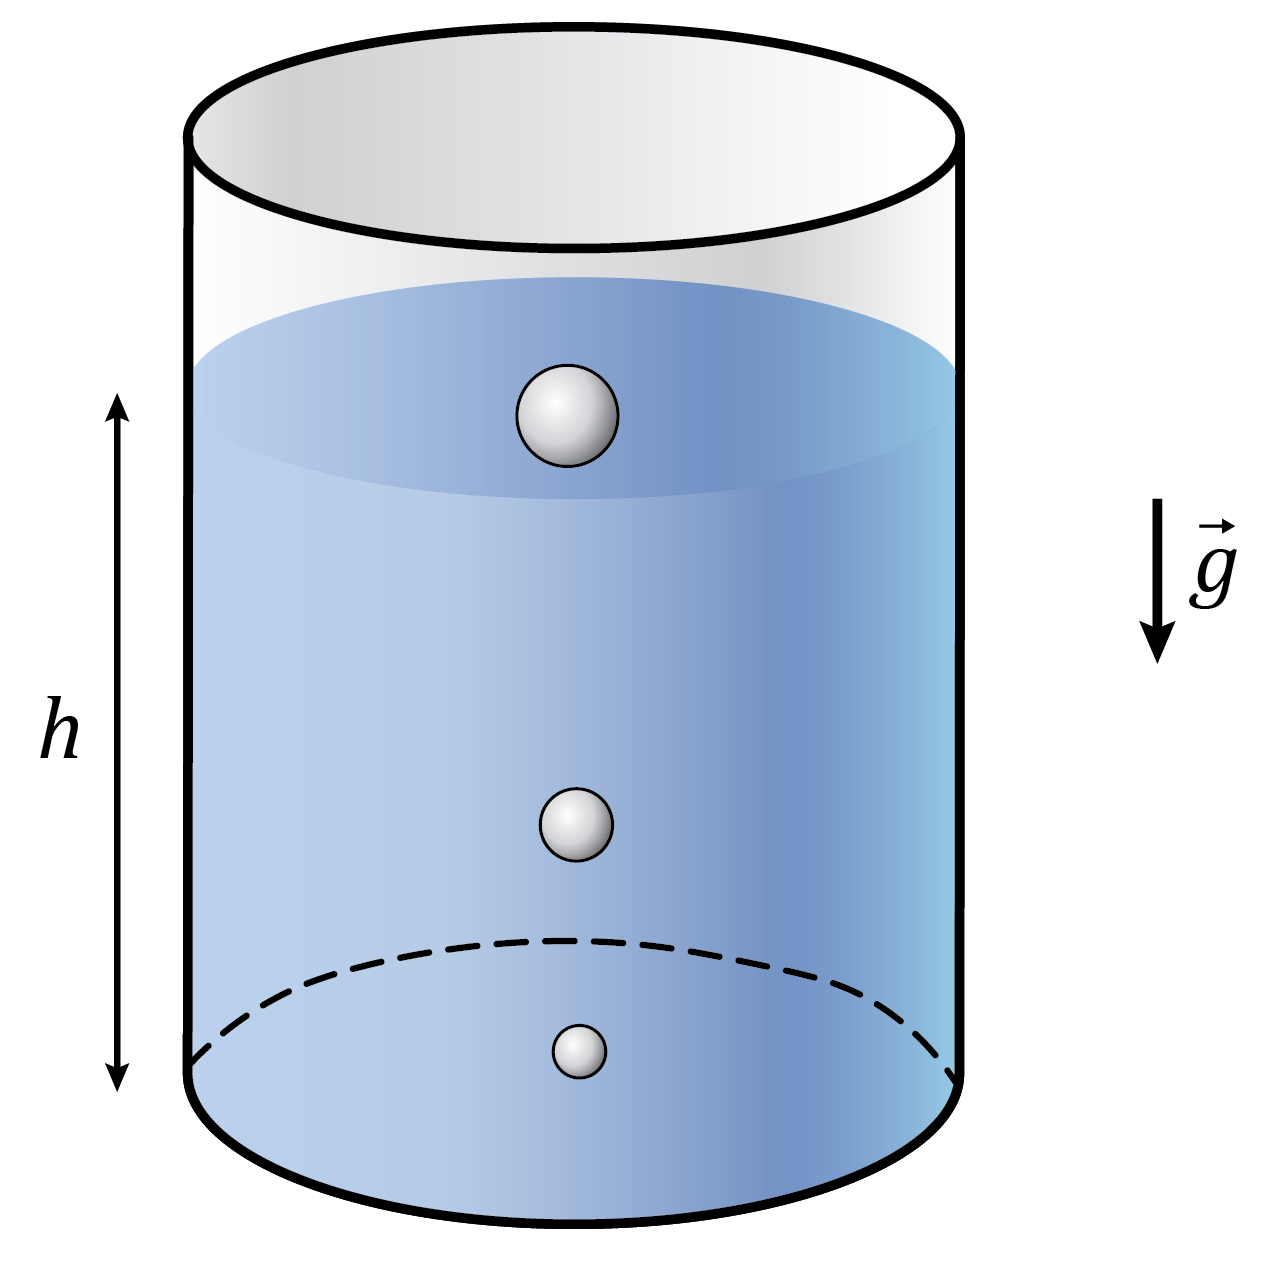
\includegraphics[height=4cm]{Images/1_bbl_theory_carbonated.PNG}
\end{center}
\vspace{2mm}

Estimate amount of energy ${\Delta E}$ dissipated due to viscous effects during ascending of that bubble. For calculations use acceleration due to gravity as ${g = 9.8\;m/s^2}$. Assume that surface tension effects are negligibly small
\end{subpr}
\begin{subpr}{A2. \hfill 0.2pts.} Estimate velocity ${v_h}$ of the bubble at the distance ${h = 0.2\;m}$ from bottom of the glass
\\
For calculations use dynamic viscosity of carbonated drink as ${\eta_f = 1.0\cdot 10^{-3}Pa\cdot s}$
\end{subpr}
\begin{subpr}{A3. \hfill 1.3pts.} 
Estimate acceleration ${a_h}$ of the bubble at the distance ${h = 0.2\;m}$ from bottom of the glass. Assume that surface tension effects are negligibly small.
\end{subpr}

\begin{problem}{B. Sonoluminescence}
Sonoluminescence is a wonderful phenomena where an external acoustic wave causes disturbances in the fluid, leading to the growth and rapid collapse of bubbles in the liquid. During that bubble collapse, content of the bubble become heated to extremely high temperatures, which causes excitation of the gas with emission of light.
\begin{center} 
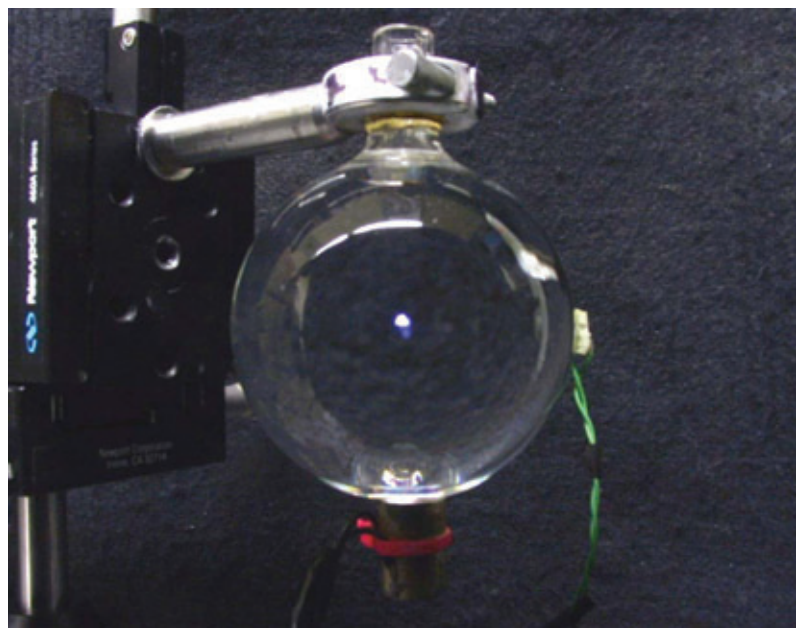
\includegraphics[height=4cm]{Images/5_bbl_theory_sonolum1.PNG}
\end{center}
\begin{center}
Photo of single bubble sonoluminescence (light blue spot in the center of glass sphere filled with fluid). Credit to Suslick K.
\end{center}
\vspace{3mm}
In this section of the problem you will have an opportunity to describe some key aspects of the sonoluminescence process
\end{problem}
\begin{subpr}{B1. \hfill 1.2pts.}
Consider a large volume of incompressible fluid of density ${\rho}$, which is initially at rest. That container with fluid has a small spherical cavity (an empty space without gas or fluid) of initial radius ${R_0}$, which starts to collapse due to an ambient fluid pressure ${P_0}$.
\begin{center} 
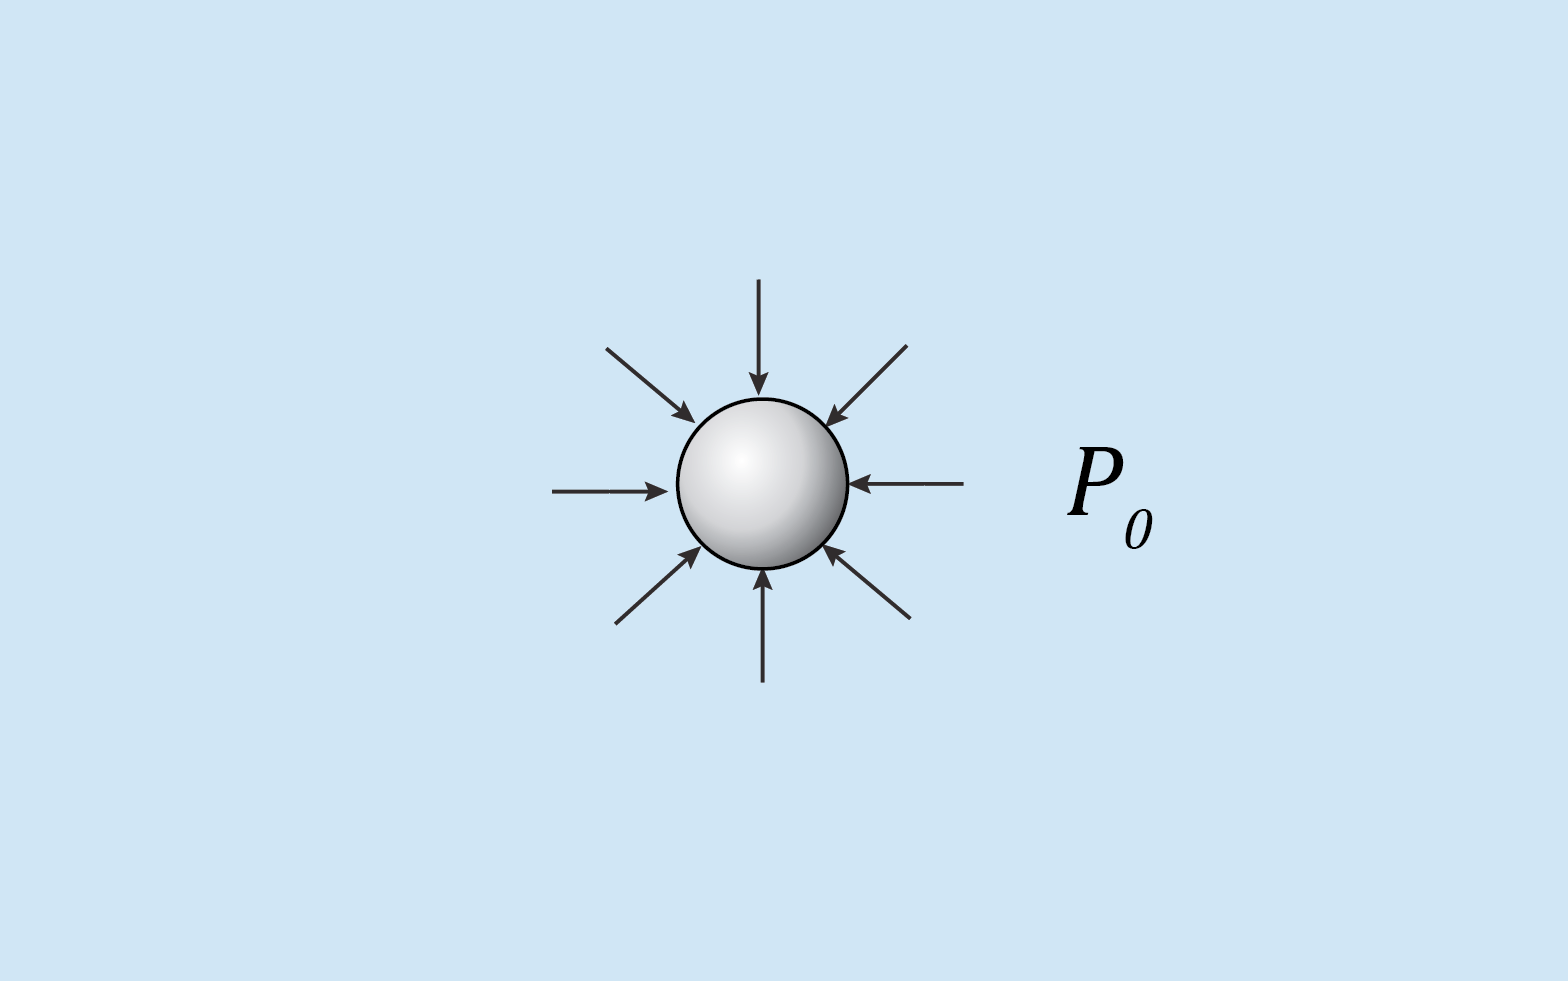
\includegraphics[height=3cm]{Images/6_bbl_prob_empty_collapse_velocity1.PNG}
\end{center}
Evaluate velocity ${v_1}$ of the boundary of cavity when radius of the bubble would decrease to some value ${R_1}$. Assume that for such small size of the cavity surface tension and viscous effects can be neglected
\end{subpr}
\begin{problem}{}
As was shown in the previous section velocity of the boundary of an empty cavity would tend to increase to infinity during collapse of the cavity at small radius ${R\!\rightarrow\! 0}.$ Thus, modeling of an empty cavity is unrealistic, which means that bubble in fluid has to be filled with some gas or vapor. This would create a counterbalance pressure inside the bubble, allowing it to bounce back at some small non-zero radius

$$	***  $$

Sonoluminescence effect occurs when changes in ambient pressure of fluid cause a bubble with noble gas to shrink, which increases temperature of the gas significantly. Usually in experiments with sonoluminescence, fluid pressure is varied as a harmonic function of time. However, here for simplicity, will consider only a rough approximation of the process, with one step of such variations in pressure, when fluid pressure is increased very fast from initial value ${P_0}$ to some new high value  ${P_f = 100P_0}$

\begin{center}
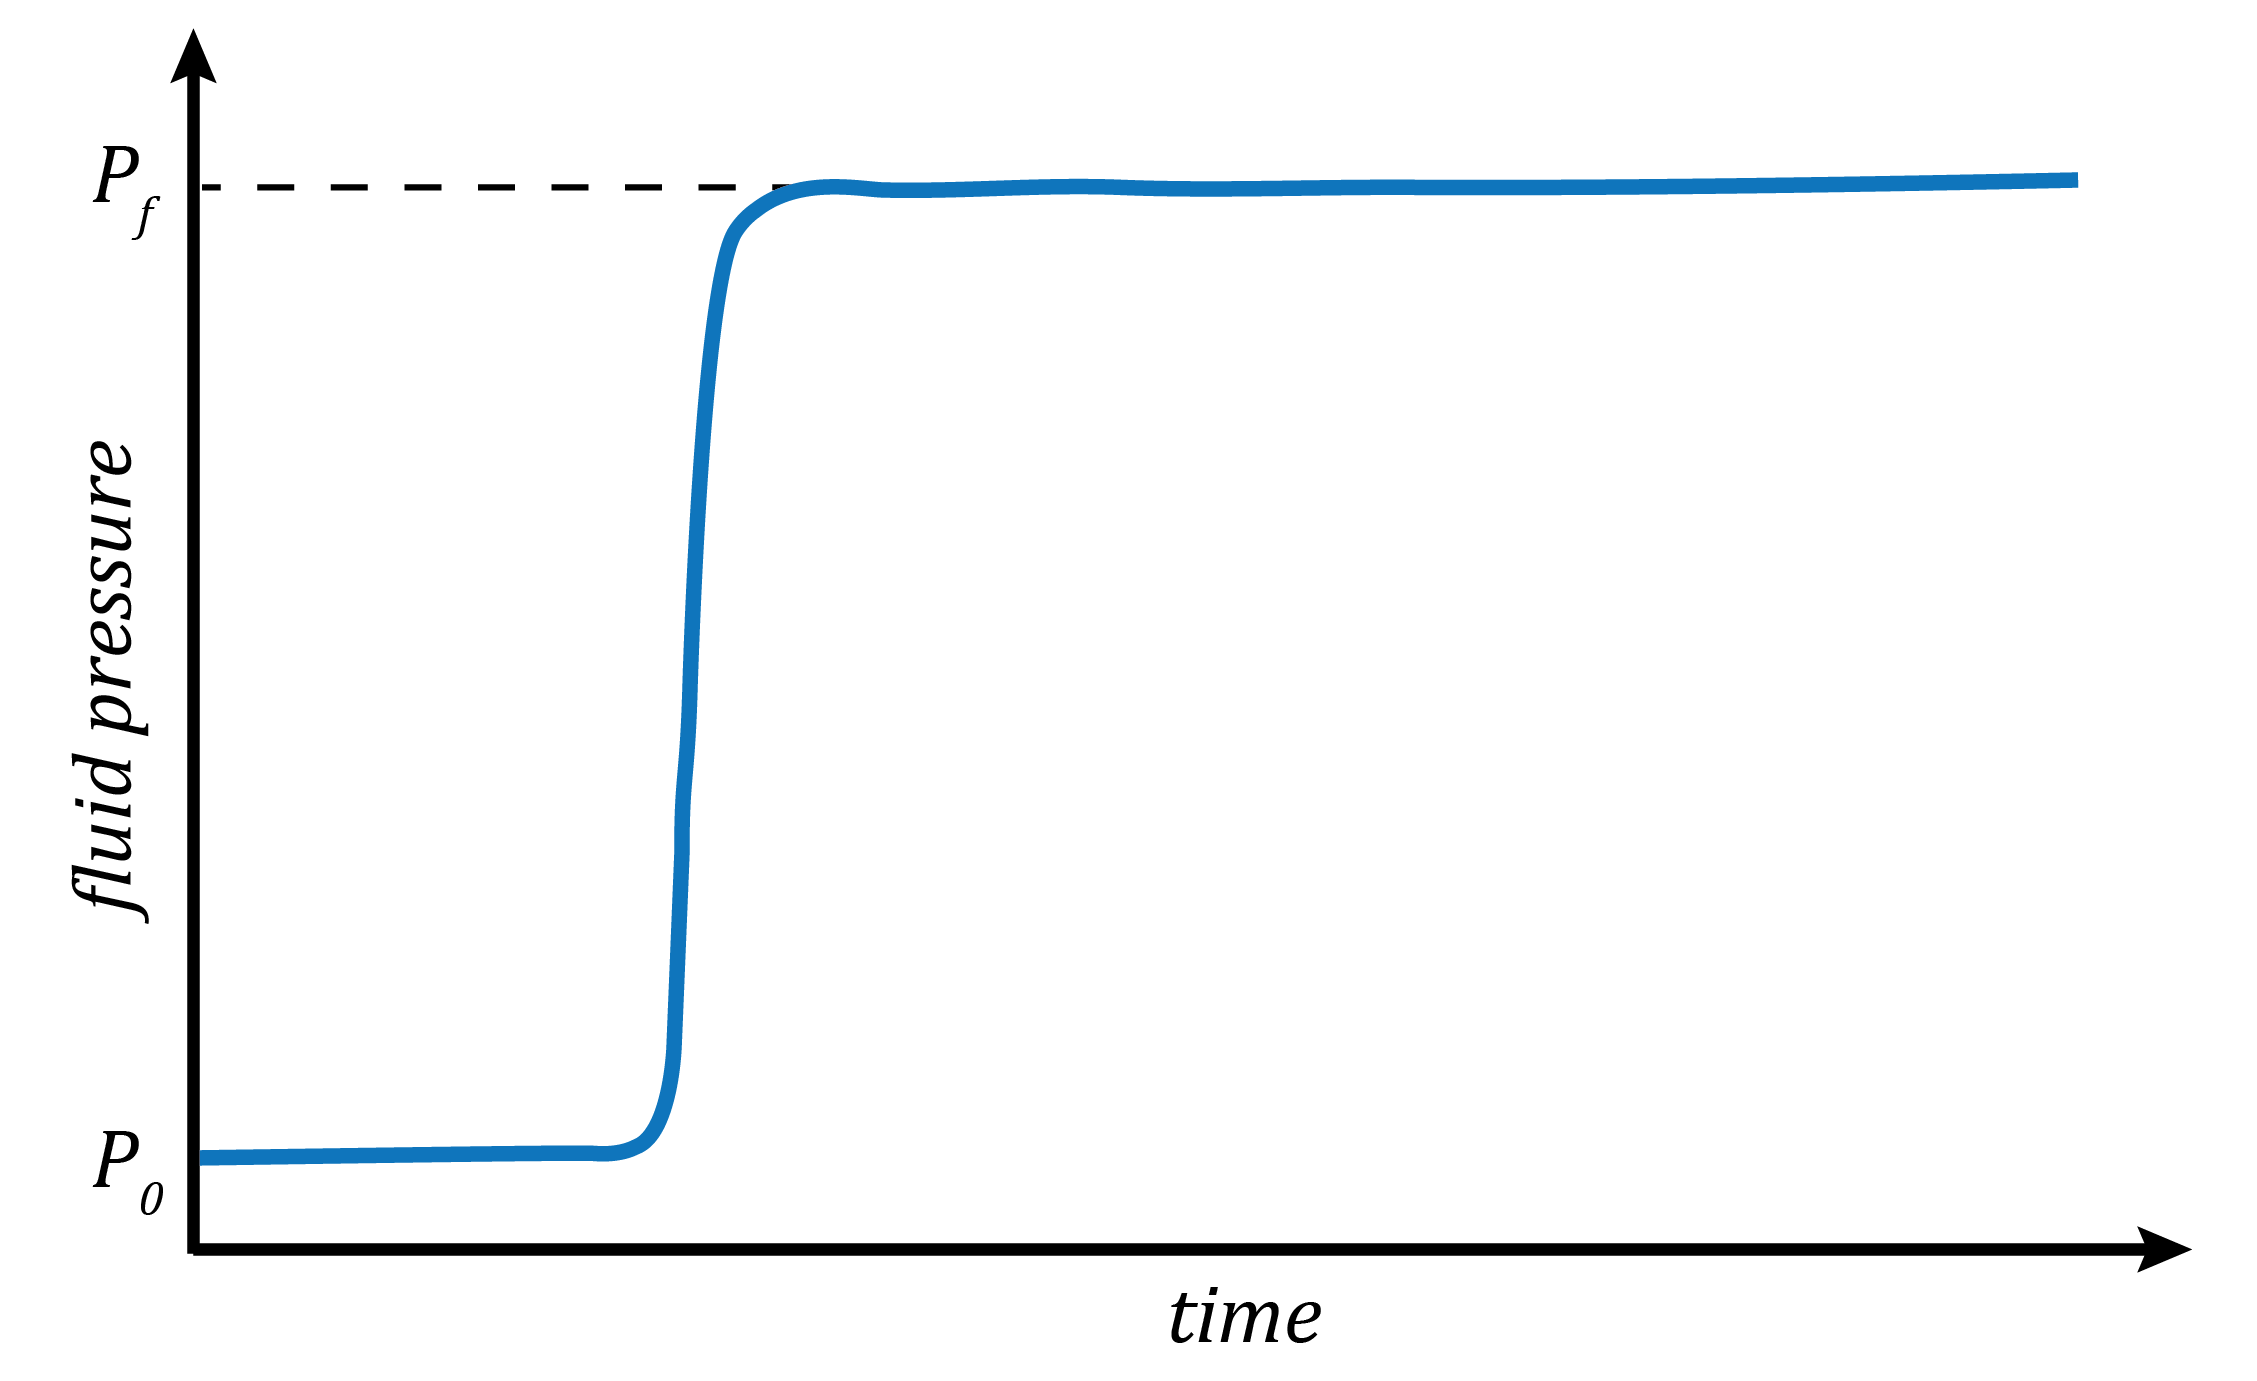
\includegraphics[width=9cm]{Images/7_bbl_theory_velocity_too_high1.PNG}
\end{center}

For the next few questions consider a bubble, which initially has a stationary radius ${R_0 = 1.0\cdot 10^{-4}\;m},$ being filled with a noble gas xenon at temperature ${T_0 = 300.0\;K}$ and pressure ${P_0}$. Shrinkage of bubble due to increased ambient fluid pressure can be accurately modeled with adiabatic process, which can be described with adiabatic constant ${\gamma}$:
$$\gamma = \frac{C_p}{C_v} = \frac{5}{3}$$
where ${C_p}$ and ${C_v}$ are molar heat capacities of xenon at constant pressure and constant volume respectively.
\end{problem}
\begin{subpr}{B2. \hfill 1.2pts.} Determine minimal radius of the bubble ${R_{min}}$ due to increase in ambient fluid pressure from ${P_0}$ to ${P_f = 100P_0}.$ Assume that surface tension and viscous friction effects can be neglected. Also for simplicity assume that presence of water vapor inside the bubble is negligibly small\\
\textbf{Note:}
For your calculations, you are not expected to use manual iterative approach for solving transcendental equations. Instead it could be easier to use calculations in some spreadsheet such as MS Excel, or write a simple script for plotting a complicated function
\end{subpr}

\begin{subpr}{B3. \hfill 0.3pts.} Evaluate maximum temperature ${T_{max}}$ of the noble gas inside cavity during its shrinkage.
\end{subpr}
\begin{problem}{Stability}

It is interesting that a lot of processes for bubbles differ based on the initial equilibrium size of the bubble. If radius of the bubble is larger than certain critical value $R_c$ , then after small disturbances in ambient fluid pressure, the bubble will start growing uncontrollably. Otherwise if initial equilibrium radius of cavity is smaller than certain threshold, it will be stable to small variations of pressure
\end{problem}

\begin{subpr}{B4. \hfill 1.2pts.} 

Consider a small bubble with radius ${R_0 = 5.0\cdot 10^{-6}m}$, which is held at pressure ${P_0 = 10^5\;Pa}$ in equilibrium with distilled water. Then fluid pressure was disturbed so that bubble expanded to radius ${R}$.
\begin{center}
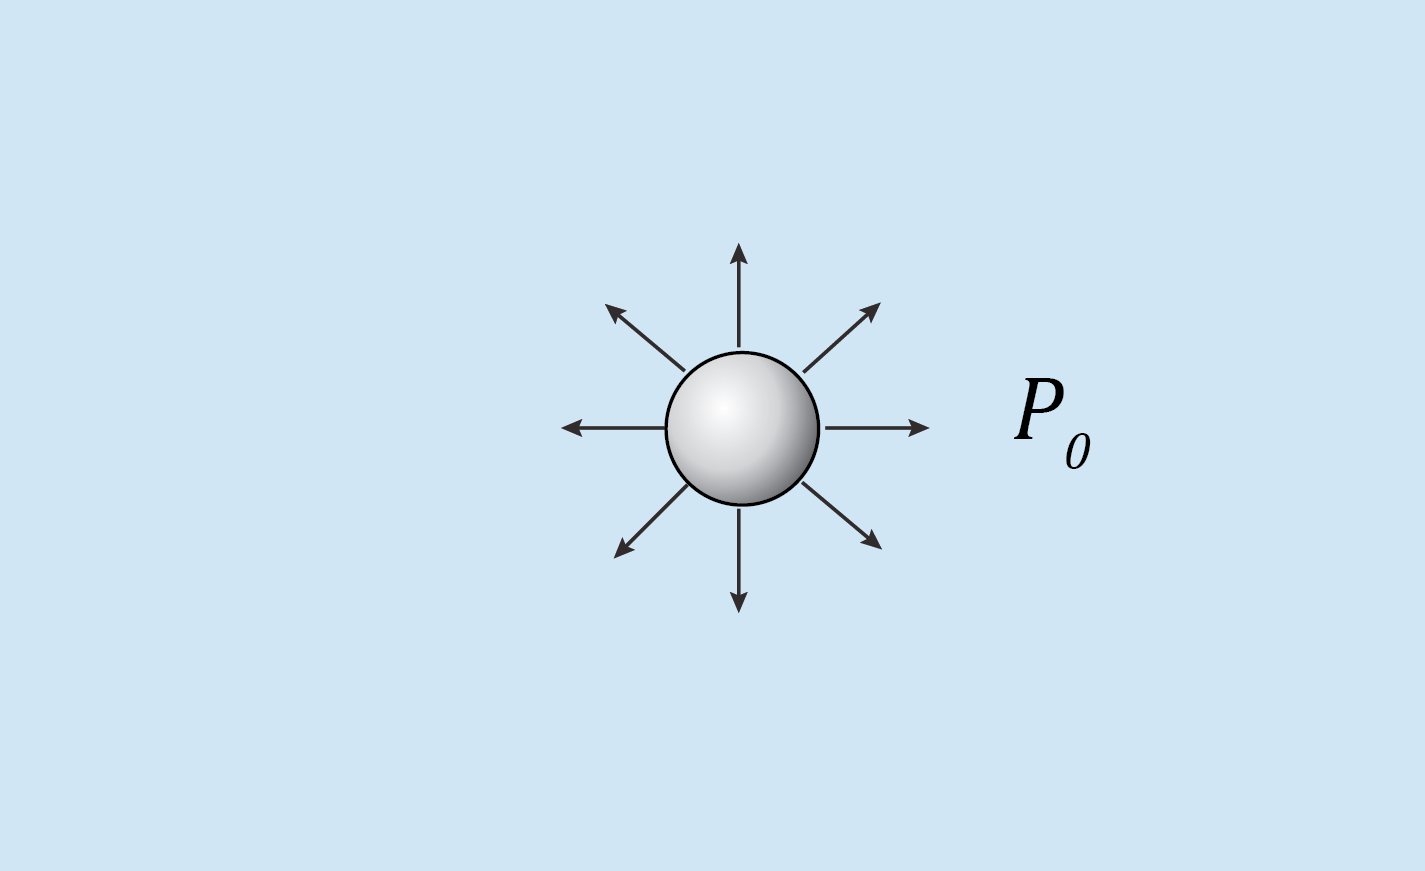
\includegraphics[height=3cm]{Images/4_bbl_prob_Blake_pressure_unstable1.PNG}
\end{center}
Calculate critical radius ${R_c}$ for this system, if entire process can be treated as isothermal, with vapor pressure at that temperature equal to ${P_v = 0.5\cdot 10^{5}\;Pa}.$ Coefficient of surface tension of water is ${\sigma = 7.2\cdot 10^{-2}N/m}$
\end{subpr}

\begin{problem}{Small oscillations}

In the next questions, assume that radius of the bubble is less than critical value ${R_c}$ unless otherwise stated. For those smaller bubbles, minor disturbances in ambient fluid pressure would cause small harmonic oscillations with frequency ${\omega}.$ That frequency can be decomposed at three components as

$$\omega^2 = \omega_p^2 + \omega_{\sigma}^2 - \omega_{\eta}^2$$
where ${\omega_p}$ is natural frequency of the bubble inside liquid, neglecting effects of surface tension and attenuation due to viscosity. While ${\omega_{\sigma}}$ and ${\omega_{\eta}}$ are additional correction terms associated with surface tension effects and viscosity respectively.
\end{problem}

\begin{subpr}{B6. \hfill 1.2pts.} Evaluate frequency ${\omega_p}$ of small harmonic oscillations of the bubble of radius ${R_0 = 1.0\cdot 10^{-4}}m$ assuming that surface tension and viscosity effects can be neglected. Consider that oscillating bubble is filled with xenon, which has adiabatic constant ${\gamma = 5/3}.$ The bubble is floating inside distilled water of density ${\rho = 1.0\cdot 10^{3}kg/m^3}.$ Assume that during those oscillations  fluid pressure ${P_f}$ is always close to initial pressure ${P_0}$ inside bubble:

$$P_f\approx P_0 = 1.0\cdot 10^{5}Pa$$

For small ${z\ll 1}$ can be used following approximation
$$(1-z)^n\approx 1-nz + \frac{n(n-1)z^2}{2}$$
\end{subpr}
\begin{subpr}{B7. \hfill 0.2pts.}
It is known that for larger bubbles with initial radius ${R_0 = 1.0\cdot 10^{-4}m}$ ratio between components of frequencies related to surface tension ${\omega_{\sigma}}$ to the frequency ${\omega_p}$ calculated with neglecting surface tension and viscous effects is
$$z_{\sigma 0} = \frac{\omega_{\sigma0}}{\omega_{p0}} = 0.1$$
Determine ratio ${z_{\sigma 1} = \omega_{\sigma 1}/\omega_{p1}}$ for a smaller bubble with radius ${R_1 = R_0/10}$
\end{subpr}
\begin{subpr}{B8. \hfill 0.3pts.}
It is known that for bubble with radius ${R_0 = 1.0\cdot 10^{-4}m}$ ratio between components of frequency related to viscous forces ${\omega_{\eta}}$ to frequency ${\omega_{p}}$ calculated by neglecting surface tension and viscous effects is
$$z_{\eta 0} = \frac{\omega_{\eta 0}}{\omega_{p0}} = 4.0\cdot 10^{-4}$$
Estimate similar ratio ${z_{\eta 1} = \frac{\omega_{\eta 1}}{\omega_{p1}}}$ for bubble with smaller radius ${R_1 = R_0/10}$
\end{subpr}
\begin{problem}{Forces due to variable pressure}
In case when pressure is spatially varied, effective force applied on the object inside such pressure field would be non-zero. For example, hydro static pressure varies with depth, creating buoyancy force in the vertical direction. In this section we will describe horizontal forces exerted on bubbles in fluid in the presence of variable pressure
\end{problem}
\begin{subpr}{B9. \hfill 0.2pts.}

Consider a small cylinder with a height ${h}$ and cross-sectional area is ${S}$ placed inside a fluid, which has spatially varied pressure ${P}$ characterized with coordinate ${x}$ as
	$$P = P_0(1+c_1x^2)$$
where ${c_1}$ is some known constant
\begin{center}
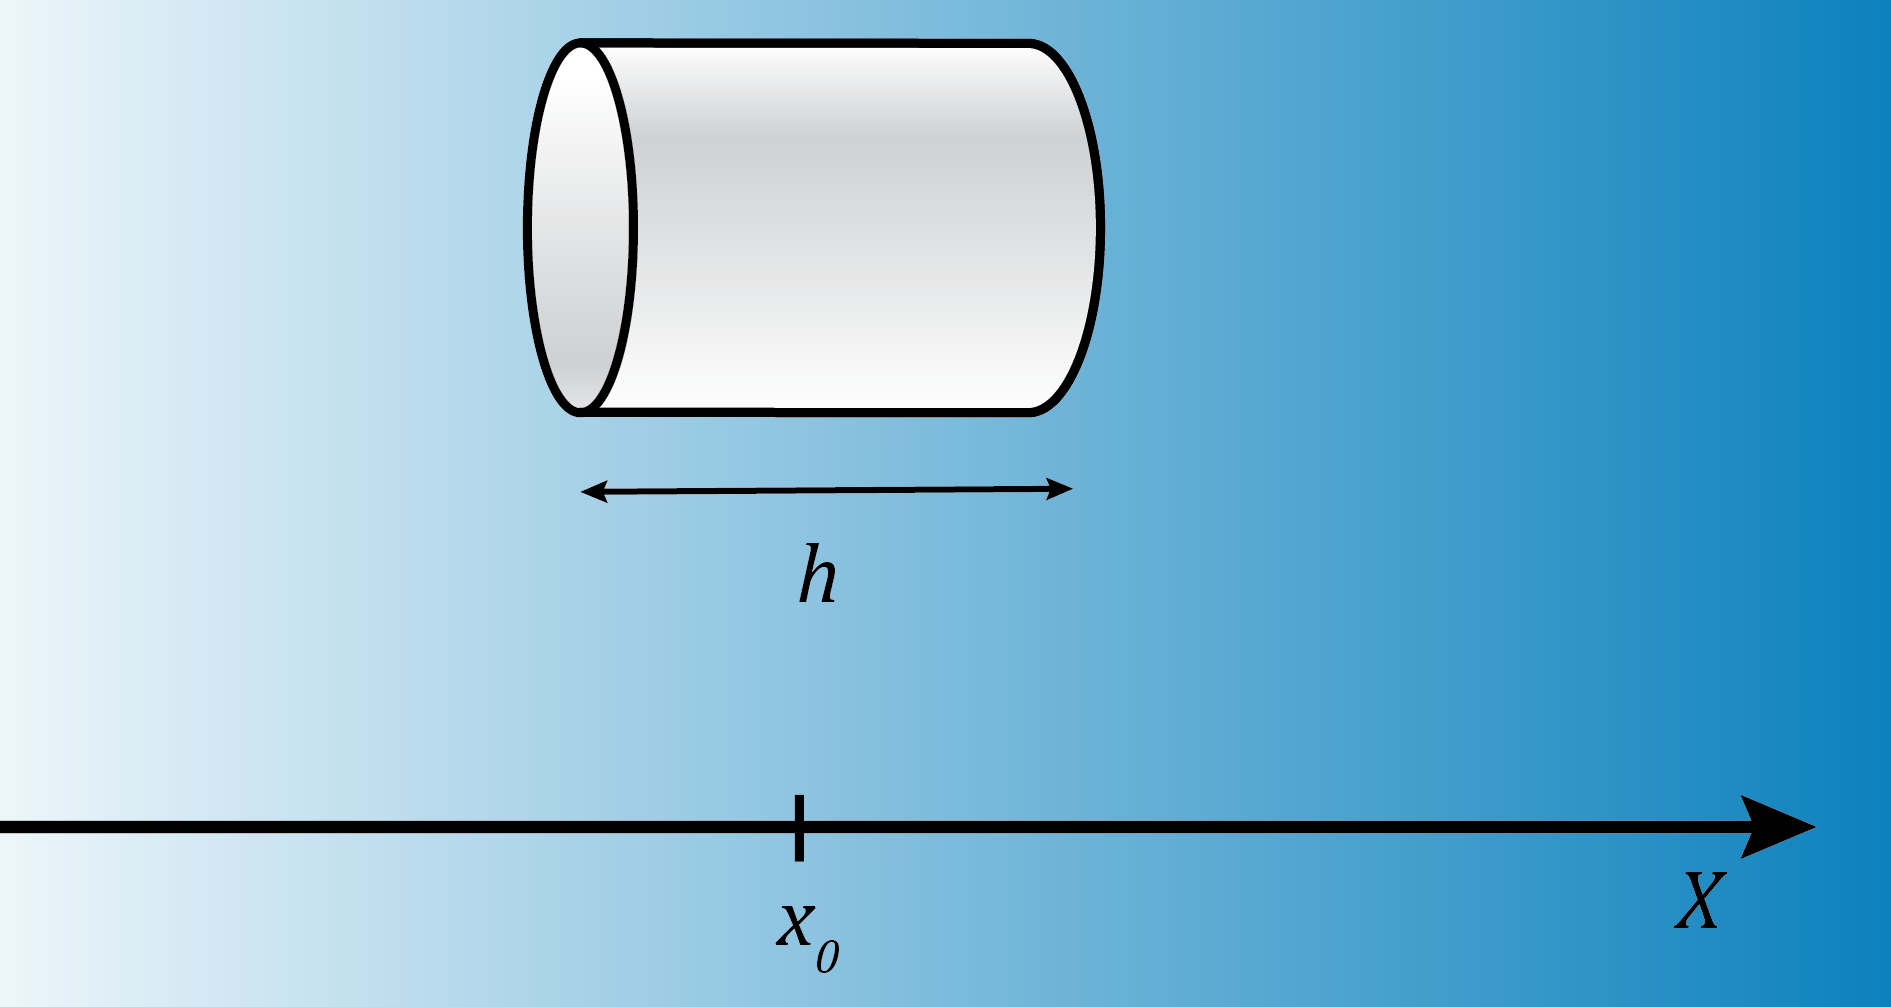
\includegraphics[height=3cm]{Images/17_bbl_prob_cylinder_cx21.PNG}
\end{center}
Center of the cylinder is located at the coordinate ${x_0\gg h},$ while main axis of the cylinder is parallel to the ${X}$ axis. Evaluate effective horizontal force ${F_x}$ exerted on this cylinder from fluid 
\end{subpr}

\begin{subpr}{B10. \hfill 0.5pts.} 
A rigid sphere of radius ${R}$ is placed inside a fluid, with variable pressure, which changes with horizontal coordinate ${x}$ as

$$P = P_0(1+c_1x^2)$$
where ${c_1}$ is some known constant\\
Center of the sphere is located at coordinate ${x_0\ll R}$. Determine effective horizontal force ${F_x}$ applied to the sphere from the surrounding fluid 
\end{subpr}

\begin{subpr}{B11. \hfill 0.2pts.}
Now consider a similar case with a rigid sphere of radius ${R}$ placed inside fluid, where pressure ${P_f}$ changes with horizontal coordinate ${x}$ and time ${t}$ as

$$P_f = P_0 + c_2\sin kx\cos\omega t$$
where ${P_0}$, ${c_2},$ ${k}$ and ${\omega}$ are known constants\\
Evaluate average effective horizontal force ${\left<F_x\right>}$ exerted at the sphere, if known that radius of the sphere is much smaller than parameter ${1/k}$
\end{subpr}

\begin{subpr}{B12. \hfill 0.3pts.} Now consider an oscillating bubble in a standing wave, with fluid pressure described as a function of horizontal coordinate ${x}$ and time ${t}$ as
$$P = P_0 + c_2\sin kx\cos\omega t$$
where ${P_0}$, ${c_2}$, ${k}$, ${\omega}$ and ${\phi}$ are some positive constants\\
It can be shown that in such variable pressure, radius of the bubble ${R}$ would change as a function of time as 
$$R = R_0 - \delta \sin kx\cos(\omega t +\phi)$$
where ${R_0}$ and ${\delta}$ are some positive constants\\
Let's call bubbles with size larger than critical radius  ${R_c}$ as "Large" and bubbles with radii smaller than ${R_c}$ as "Small". It can be shown that parameter ${\phi}$ is equal ${0}$ or ${\pi}$\\
Let ${\phi_L}$ and ${\phi_S}$ are coefficients ${\phi}$ for "Large" and "Small" bubbles respectively. Briefly justify in 1-2 sentences or in a few short equations, which values ${0}$ or ${\pi}$ should we use for parameters ${\phi_L}$ and ${\phi_S}$
\end{subpr}
\begin{subpr}{B13. \hfill 0.7pts.} 
Consider bubble described in the question ${B12}$ with small oscillations such that ${\delta \ll R_0}$. Determine average horizontal force ${\left<F_x\right>}$ exerted at this oscillating bubble
\end{subpr}
\begin{subpr}{B14. \hfill 0.5pts.}
Consider that fluid pressure changes with time ${t}$ and coordinate ${x}$ as
$$	P = P_0 + c_3\sin kx\cos\omega t$$
This is an equation of a standing wave, which can be characterized with "nodes" and "antinodes"
\begin{center}
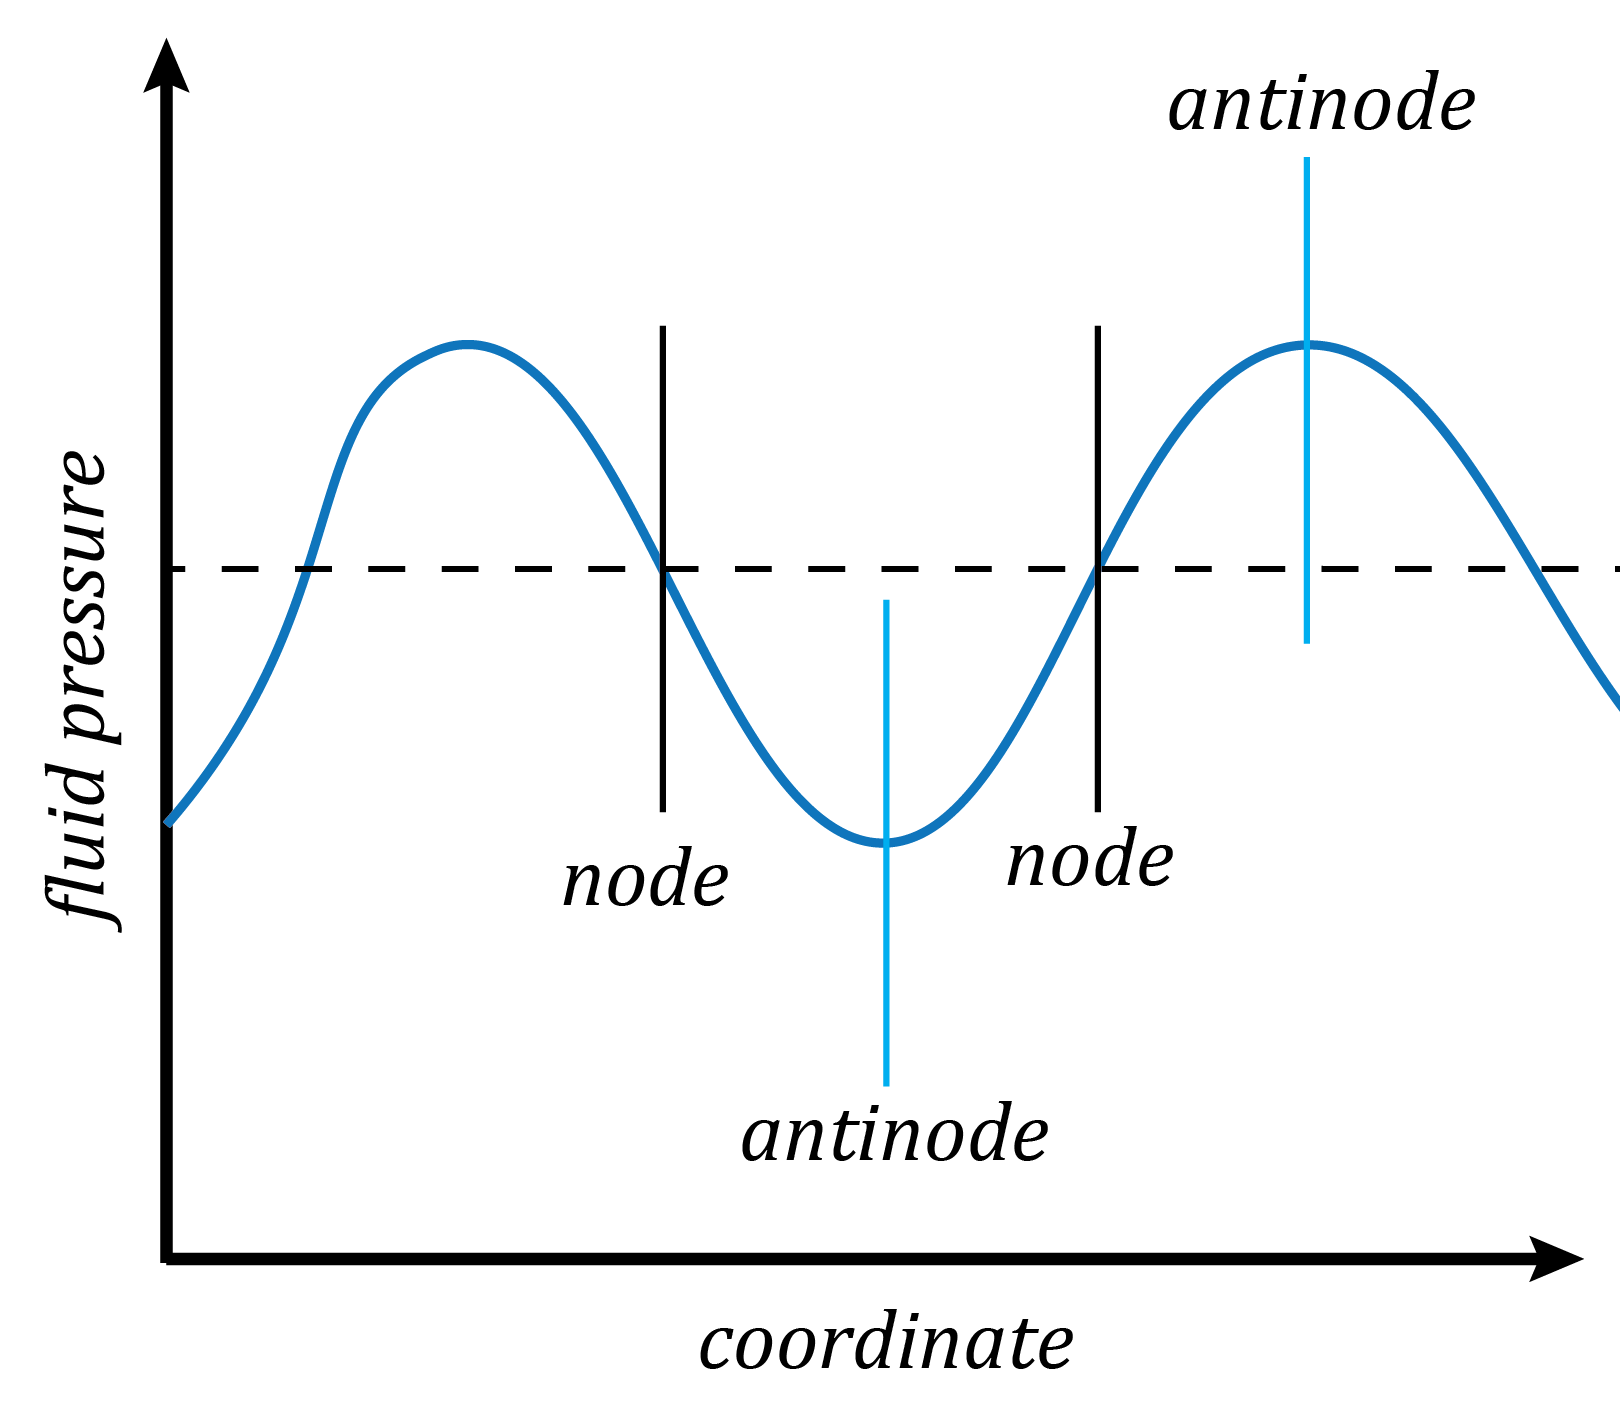
\includegraphics[height=3cm]{Images/22_bbl_prob_nodes_antinodes_grouping1.PNG}
\end{center}
Describe briefly in ${1-2}$ sentences where would gather "Large" and "Small" bubble in that standing wave (either close to nodes or in the vicinity of antinodes)	
\end{subpr}

\clearpage